% ============================================================================
% AgriPerceiver: ICML 2026 Workshop Paper
% 3rd Workshop on Multi-modal Foundation Models and LLMs for Life Sciences
% ============================================================================
\documentclass{article}

% ICML 2026 workshop style — replace with official .sty when available
\usepackage[accepted]{icml2024}  % Use latest available ICML style

\usepackage{amsmath,amssymb,amsfonts}
\usepackage{graphicx}
\usepackage{booktabs}
\usepackage{multirow}
\usepackage{xcolor}
\usepackage{hyperref}
\usepackage{cleveref}
\usepackage{subcaption}
\usepackage{enumitem}
\usepackage{tikz}
\usetikzlibrary{positioning, arrows.meta, fit, backgrounds, calc, shapes.geometric}

% ── Colors ─────────────────────────────────────────────────────────────────────
\definecolor{visionblue}{HTML}{2563EB}
\definecolor{bridgeorange}{HTML}{F59E0B}
\definecolor{llmred}{HTML}{DC2626}
\definecolor{lightgray}{HTML}{F3F4F6}

% ── Macros ─────────────────────────────────────────────────────────────────────
\newcommand{\ours}{AgriPerceiver}
\newcommand{\perceiverr}{Perceiver Resampler}
\newcommand{\siglip}{SigLIP-SO400M}
\newcommand{\phithree}{Phi-3-mini-128k}
\newcommand{\ie}{\textit{i.e.}}
\newcommand{\eg}{\textit{e.g.}}
\newcommand{\cf}{\textit{cf.}}
\newcommand{\etc}{\textit{etc.}}

\icmltitlerunning{AgriPerceiver: Perceiver-Based VLM for Agricultural Pathology}

\begin{document}

\twocolumn[
\icmltitle{AgriPerceiver: A Perceiver-Based Vision-Language Model \\
for Structured Agricultural Pathology Diagnosis}

% Authors — update before submission
\icmlsetsymbol{equal}{*}

\begin{icmlauthorlist}
\icmlauthor{Author One}{inst1}
\icmlauthor{Author Two}{inst1}
\end{icmlauthorlist}

\icmlaffiliation{inst1}{Department of Computer Science, University Name}

\icmlcorrespondingauthor{Author One}{author@university.edu}

\icmlkeywords{Vision-Language Models, Agricultural AI, Perceiver, Plant Pathology}

\vskip 0.3in
]

\printAffiliationsAndNotice{}

% ╔═══════════════════════════════════════════════════════════════════════════╗
% ║ ABSTRACT                                                                 ║
% ╚═══════════════════════════════════════════════════════════════════════════╝

\begin{abstract}
We present \ours{}, a lightweight, domain-specialized vision-language model
that generates structured JSON diagnostic reports from photographs of plant
leaves. Our architecture introduces a \emph{perception bridge} consisting of
a Perceiver Resampler that compresses 3,645 visual tokens from a frozen
SigLIP-SO400M encoder into 128 learned latents (28.5$\times$ compression),
coupled with AnyRes spatial tiling and learned tile-position embeddings.
A two-stage curriculum---alignment pretraining followed by LoRA-based
specialization---enables the frozen Phi-3-mini backbone to produce
schema-compliant diagnostic outputs covering disease identification,
severity scoring, symptom analysis, and treatment recommendations.
Trained on 101K images labeled by Gemma-3-12B-IT and evaluated with a
9-metric framework including structural validity, classification F1,
regression accuracy, BERTScore, and LLM-as-judge consensus scoring,
\ours{} demonstrates [XX\% composite score], outperforming general-purpose
VLMs while using only $\sim$2\% trainable parameters in Stage~2.
\end{abstract}

% ╔═══════════════════════════════════════════════════════════════════════════╗
% ║ 1. INTRODUCTION                                                          ║
% ╚═══════════════════════════════════════════════════════════════════════════╝

\section{Introduction}
\label{sec:intro}

Accurate and timely diagnosis of plant diseases is critical for food
security, with crop losses from pathogens estimated at 20--40\% of global
agricultural output annually~\cite{savary2019global}. While general-purpose
vision-language models (VLMs) like LLaVA~\cite{liu2024visual} and
InternVL~\cite{chen2024internvl} demonstrate impressive visual understanding,
their application to agricultural pathology is limited by:
(1)~lack of domain-specific training data with structured diagnostic labels,
(2)~inefficient visual token handling that hinders real-time deployment, and
(3)~absence of schema-constrained outputs required for integration with
agricultural decision-support systems.

We address these challenges with three contributions:

\begin{enumerate}[leftmargin=*,itemsep=2pt]
\item \textbf{Perceiver-based perception bridge}: A 28.5$\times$ visual
      token compression mechanism that maintains spatial fidelity through
      AnyRes tiling and learned tile-position embeddings while reducing
      computational cost for the language model.

\item \textbf{Two-stage training curriculum}: Alignment pretraining of the
      bridge ($\sim$50M parameters) followed by LoRA specialization
      ($\sim$35M adapters, $r{=}32$), keeping the 3.8B-parameter Phi-3
      backbone largely frozen.

\item \textbf{Automated data pipeline and evaluation framework}: A
      Gemma-3-12B-IT-based labeling pipeline producing 101K structured
      annotations, validated with a 9-metric evaluation suite including
      multi-judge LLM consensus scoring.
\end{enumerate}

% ╔═══════════════════════════════════════════════════════════════════════════╗
% ║ 2. RELATED WORK                                                          ║
% ╚═══════════════════════════════════════════════════════════════════════════╝

\section{Related Work}
\label{sec:related}

\paragraph{Vision-Language Models for Science.}
Recent VLMs including LLaVA-NeXT~\cite{liu2024llavanext},
InternVL2~\cite{chen2024internvl}, and Gemma-3~\cite{team2024gemma}
have shown strong general visual reasoning but limited domain expertise
in specialized fields. BioMedCLIP~\cite{zhang2023biomedclip} targets
biomedical imaging, but agricultural pathology remains underserved.

\paragraph{Perceiver Architectures.}
The Perceiver~\cite{jaegle2021perceiver} and Perceiver
Resampler~\cite{alayrac2022flamingo} demonstrate that cross-attention
with learned latent queries can efficiently compress heterogeneous inputs.
We adapt this mechanism for multi-tile visual features with spatial
position encoding.

\paragraph{Efficient Fine-tuning.}
LoRA~\cite{hu2022lora} and QLoRA~\cite{dettmers2024qlora} enable
parameter-efficient adaptation of large models. Our two-stage approach
separates modality alignment from task specialization, following the
curriculum established by LLaVA~\cite{liu2024visual}.

% ╔═══════════════════════════════════════════════════════════════════════════╗
% ║ 3. METHOD                                                                ║
% ╚═══════════════════════════════════════════════════════════════════════════╝

\section{Method}
\label{sec:method}

\subsection{Architecture Overview}

\ours{} (\Cref{fig:architecture}) consists of four components:
(1)~a frozen SigLIP-SO400M vision encoder,
(2)~a perception bridge comprising TileEmbeddings, VisionProjector,
and PerceiverResampler,
(3)~a splice-and-forward injection mechanism, and
(4)~a Phi-3-mini-128k language model with LoRA adapters.

% ── AgriPerceiver Architecture Diagram (TikZ) ─────────────────────────────
% Include in main.tex with: % ── AgriPerceiver Architecture Diagram (TikZ) ─────────────────────────────
% Include in main.tex with: % ── AgriPerceiver Architecture Diagram (TikZ) ─────────────────────────────
% Include in main.tex with: \input{figures/architecture_tikz}

\begin{figure*}[t]
\centering
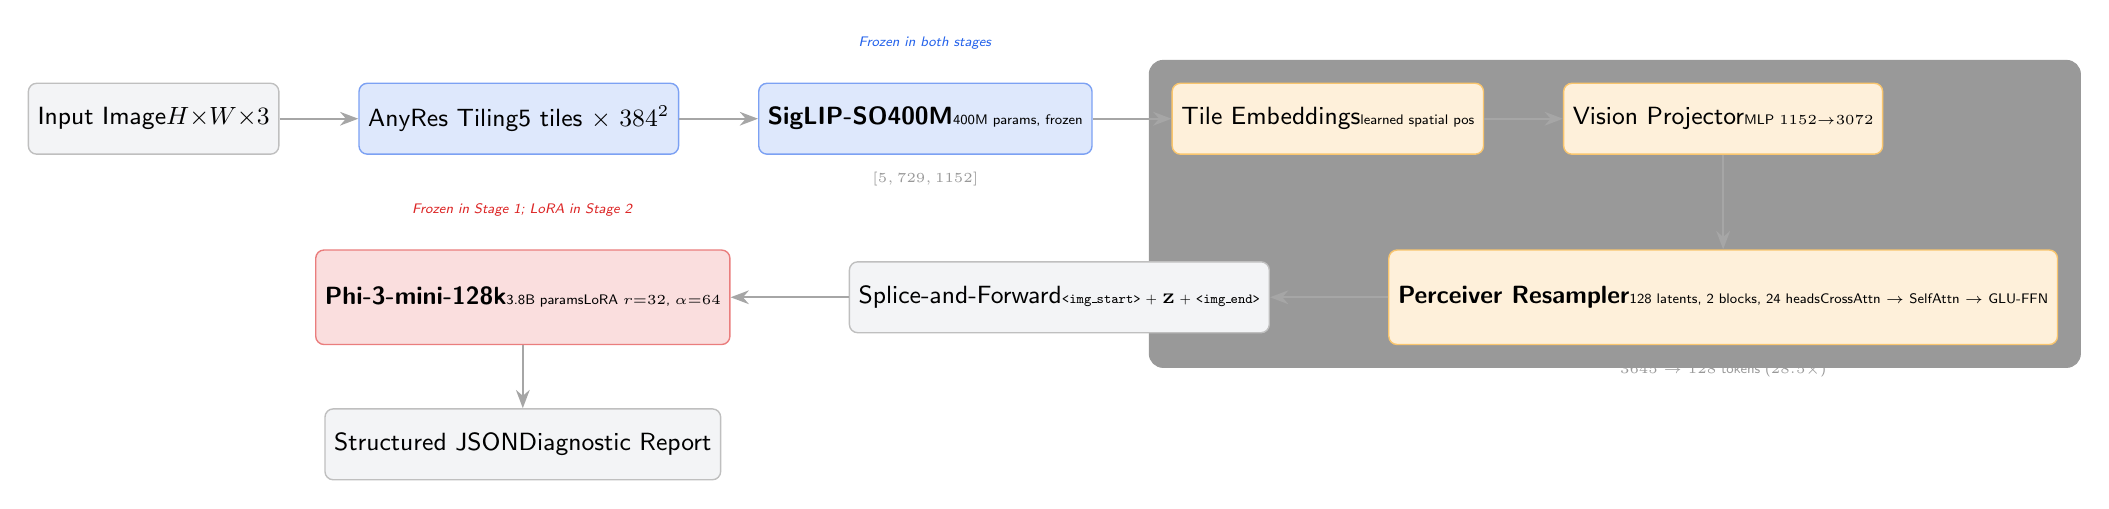
\begin{tikzpicture}[
    >=Stealth,
    node distance=0.6cm and 1.0cm,
    block/.style={
        rectangle, draw, rounded corners=3pt, minimum height=0.9cm,
        text centered, font=\small\sffamily, line width=0.5pt
    },
    vblock/.style={block, fill=visionblue!15, draw=visionblue!60},
    bblock/.style={block, fill=bridgeorange!15, draw=bridgeorange!60},
    lblock/.style={block, fill=llmred!15, draw=llmred!60},
    gblock/.style={block, fill=lightgray, draw=gray!50},
    arrow/.style={->, thick, color=gray!70},
    label/.style={font=\tiny\sffamily, color=gray!80},
]

% ── Input ──────────────────────────────────────────────────────────────────
\node[gblock, minimum width=2.2cm] (input) {Input Image\\$H{\times}W{\times}3$};

% ── AnyRes Tiling ─────────────────────────────────────────────────────────
\node[vblock, right=1.0cm of input, minimum width=2.4cm] (tiling)
    {AnyRes Tiling\\5 tiles $\times$ $384^2$};

% ── SigLIP ────────────────────────────────────────────────────────────────
\node[vblock, right=1.0cm of tiling, minimum width=2.8cm] (siglip)
    {\textbf{SigLIP-SO400M}\\{\tiny 400M params, frozen}};
\node[label, below=0.1cm of siglip] {$[5, 729, 1152]$};

% ── Tile Embeddings ───────────────────────────────────────────────────────
\node[bblock, right=1.0cm of siglip, minimum width=2.4cm] (tile_emb)
    {Tile Embeddings\\{\tiny learned spatial pos}};

% ── Vision Projector ──────────────────────────────────────────────────────
\node[bblock, right=1.0cm of tile_emb, minimum width=2.4cm] (projector)
    {Vision Projector\\{\tiny MLP $1152{\to}3072$}};
\node[label, below=0.1cm of projector] {$[3645, 3072]$};

% ── Perceiver Resampler ──────────────────────────────────────────────────
\node[bblock, below=1.2cm of projector, minimum width=3.0cm, minimum height=1.2cm]
    (perceiver) {\textbf{Perceiver Resampler}\\{\tiny 128 latents, 2 blocks, 24 heads}\\{\tiny CrossAttn $\to$ SelfAttn $\to$ GLU-FFN}};
\node[label, below=0.1cm of perceiver] {$3645 \to 128$ tokens ($28.5\times$)};

% ── Splice-and-Forward ───────────────────────────────────────────────────
\node[gblock, left=1.5cm of perceiver, minimum width=2.8cm] (splice)
    {Splice-and-Forward\\{\tiny \texttt{<img\_start>} + $\mathbf{Z}$ + \texttt{<img\_end>}}};

% ── Phi-3 ────────────────────────────────────────────────────────────────
\node[lblock, left=1.5cm of splice, minimum width=3.0cm, minimum height=1.2cm]
    (phi3) {\textbf{Phi-3-mini-128k}\\{\tiny 3.8B params}\\{\tiny LoRA $r{=}32$, $\alpha{=}64$}};

% ── Output ───────────────────────────────────────────────────────────────
\node[gblock, below=0.8cm of phi3, minimum width=2.8cm] (output)
    {Structured JSON\\Diagnostic Report};

% ── Arrows ───────────────────────────────────────────────────────────────
\draw[arrow] (input) -- (tiling);
\draw[arrow] (tiling) -- (siglip);
\draw[arrow] (siglip) -- (tile_emb);
\draw[arrow] (tile_emb) -- (projector);
\draw[arrow] (projector) -- (perceiver);
\draw[arrow] (perceiver) -- (splice);
\draw[arrow] (splice) -- (phi3);
\draw[arrow] (phi3) -- (output);

% ── Brace for Perception Bridge ─────────────────────────────────────────
\begin{scope}[on background layer]
    \node[draw=bridgeorange!40, fill=bridgeorange!5, rounded corners=5pt,
          fit=(tile_emb)(projector)(perceiver), inner sep=8pt,
          label={[font=\small\sffamily\bfseries, text=bridgeorange!80]above:Perception Bridge ($\sim$50M)}] {};
\end{scope}

% ── Stage labels ─────────────────────────────────────────────────────────
\node[font=\tiny\sffamily, color=visionblue, above=0.3cm of siglip]
    {\textit{Frozen in both stages}};
\node[font=\tiny\sffamily, color=llmred, above=0.3cm of phi3]
    {\textit{Frozen in Stage 1; LoRA in Stage 2}};

\end{tikzpicture}
\caption{\textbf{AgriPerceiver architecture.} An input leaf image is
tiled into 5 spatial regions, encoded by frozen SigLIP-SO400M, enriched
with learned tile-position embeddings, projected to the LLM dimension,
and compressed from 3,645 to 128 tokens by the Perceiver Resampler.
The compressed latents are spliced into Phi-3-mini's input sequence
for autoregressive generation of structured diagnostic JSON.}
\label{fig:architecture}
\end{figure*}


\begin{figure*}[t]
\centering
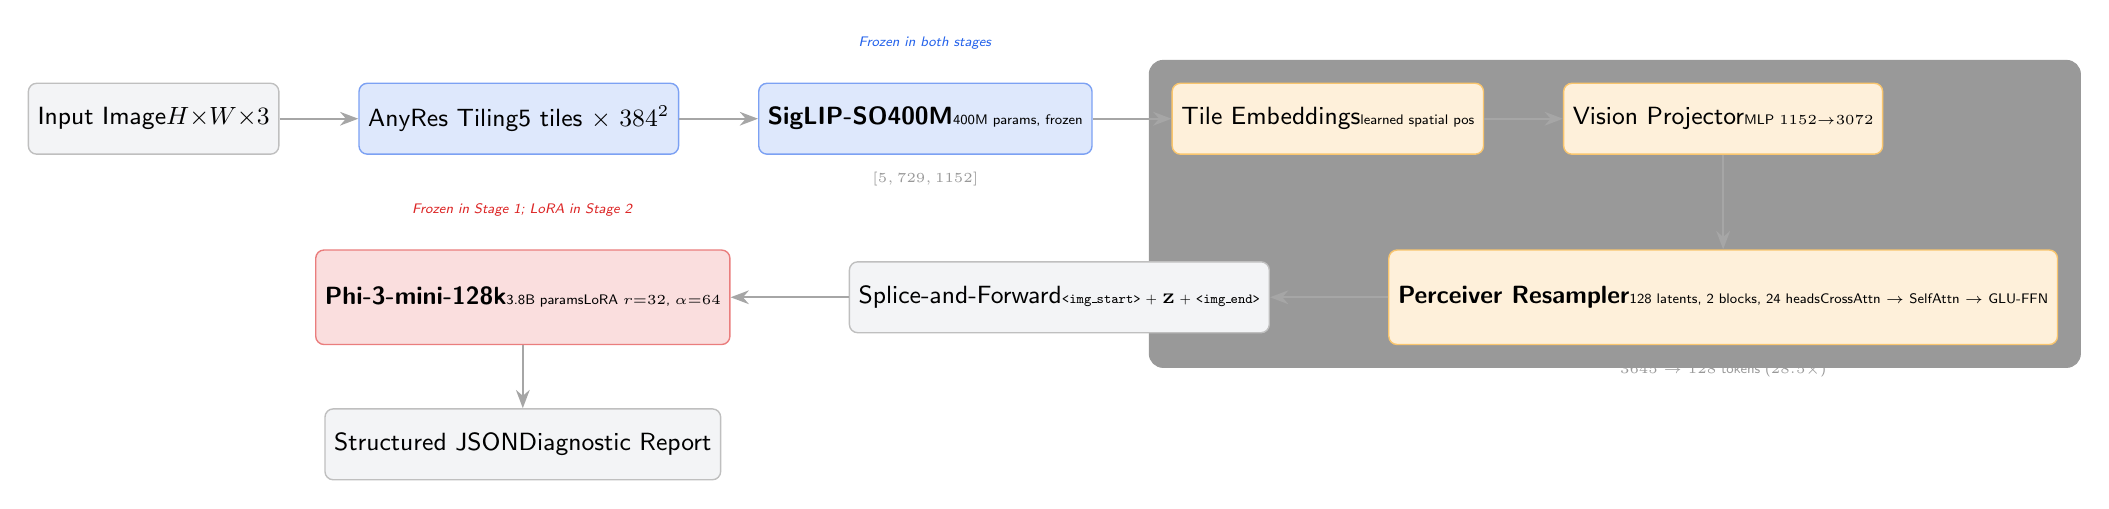
\begin{tikzpicture}[
    >=Stealth,
    node distance=0.6cm and 1.0cm,
    block/.style={
        rectangle, draw, rounded corners=3pt, minimum height=0.9cm,
        text centered, font=\small\sffamily, line width=0.5pt
    },
    vblock/.style={block, fill=visionblue!15, draw=visionblue!60},
    bblock/.style={block, fill=bridgeorange!15, draw=bridgeorange!60},
    lblock/.style={block, fill=llmred!15, draw=llmred!60},
    gblock/.style={block, fill=lightgray, draw=gray!50},
    arrow/.style={->, thick, color=gray!70},
    label/.style={font=\tiny\sffamily, color=gray!80},
]

% ── Input ──────────────────────────────────────────────────────────────────
\node[gblock, minimum width=2.2cm] (input) {Input Image\\$H{\times}W{\times}3$};

% ── AnyRes Tiling ─────────────────────────────────────────────────────────
\node[vblock, right=1.0cm of input, minimum width=2.4cm] (tiling)
    {AnyRes Tiling\\5 tiles $\times$ $384^2$};

% ── SigLIP ────────────────────────────────────────────────────────────────
\node[vblock, right=1.0cm of tiling, minimum width=2.8cm] (siglip)
    {\textbf{SigLIP-SO400M}\\{\tiny 400M params, frozen}};
\node[label, below=0.1cm of siglip] {$[5, 729, 1152]$};

% ── Tile Embeddings ───────────────────────────────────────────────────────
\node[bblock, right=1.0cm of siglip, minimum width=2.4cm] (tile_emb)
    {Tile Embeddings\\{\tiny learned spatial pos}};

% ── Vision Projector ──────────────────────────────────────────────────────
\node[bblock, right=1.0cm of tile_emb, minimum width=2.4cm] (projector)
    {Vision Projector\\{\tiny MLP $1152{\to}3072$}};
\node[label, below=0.1cm of projector] {$[3645, 3072]$};

% ── Perceiver Resampler ──────────────────────────────────────────────────
\node[bblock, below=1.2cm of projector, minimum width=3.0cm, minimum height=1.2cm]
    (perceiver) {\textbf{Perceiver Resampler}\\{\tiny 128 latents, 2 blocks, 24 heads}\\{\tiny CrossAttn $\to$ SelfAttn $\to$ GLU-FFN}};
\node[label, below=0.1cm of perceiver] {$3645 \to 128$ tokens ($28.5\times$)};

% ── Splice-and-Forward ───────────────────────────────────────────────────
\node[gblock, left=1.5cm of perceiver, minimum width=2.8cm] (splice)
    {Splice-and-Forward\\{\tiny \texttt{<img\_start>} + $\mathbf{Z}$ + \texttt{<img\_end>}}};

% ── Phi-3 ────────────────────────────────────────────────────────────────
\node[lblock, left=1.5cm of splice, minimum width=3.0cm, minimum height=1.2cm]
    (phi3) {\textbf{Phi-3-mini-128k}\\{\tiny 3.8B params}\\{\tiny LoRA $r{=}32$, $\alpha{=}64$}};

% ── Output ───────────────────────────────────────────────────────────────
\node[gblock, below=0.8cm of phi3, minimum width=2.8cm] (output)
    {Structured JSON\\Diagnostic Report};

% ── Arrows ───────────────────────────────────────────────────────────────
\draw[arrow] (input) -- (tiling);
\draw[arrow] (tiling) -- (siglip);
\draw[arrow] (siglip) -- (tile_emb);
\draw[arrow] (tile_emb) -- (projector);
\draw[arrow] (projector) -- (perceiver);
\draw[arrow] (perceiver) -- (splice);
\draw[arrow] (splice) -- (phi3);
\draw[arrow] (phi3) -- (output);

% ── Brace for Perception Bridge ─────────────────────────────────────────
\begin{scope}[on background layer]
    \node[draw=bridgeorange!40, fill=bridgeorange!5, rounded corners=5pt,
          fit=(tile_emb)(projector)(perceiver), inner sep=8pt,
          label={[font=\small\sffamily\bfseries, text=bridgeorange!80]above:Perception Bridge ($\sim$50M)}] {};
\end{scope}

% ── Stage labels ─────────────────────────────────────────────────────────
\node[font=\tiny\sffamily, color=visionblue, above=0.3cm of siglip]
    {\textit{Frozen in both stages}};
\node[font=\tiny\sffamily, color=llmred, above=0.3cm of phi3]
    {\textit{Frozen in Stage 1; LoRA in Stage 2}};

\end{tikzpicture}
\caption{\textbf{AgriPerceiver architecture.} An input leaf image is
tiled into 5 spatial regions, encoded by frozen SigLIP-SO400M, enriched
with learned tile-position embeddings, projected to the LLM dimension,
and compressed from 3,645 to 128 tokens by the Perceiver Resampler.
The compressed latents are spliced into Phi-3-mini's input sequence
for autoregressive generation of structured diagnostic JSON.}
\label{fig:architecture}
\end{figure*}


\begin{figure*}[t]
\centering
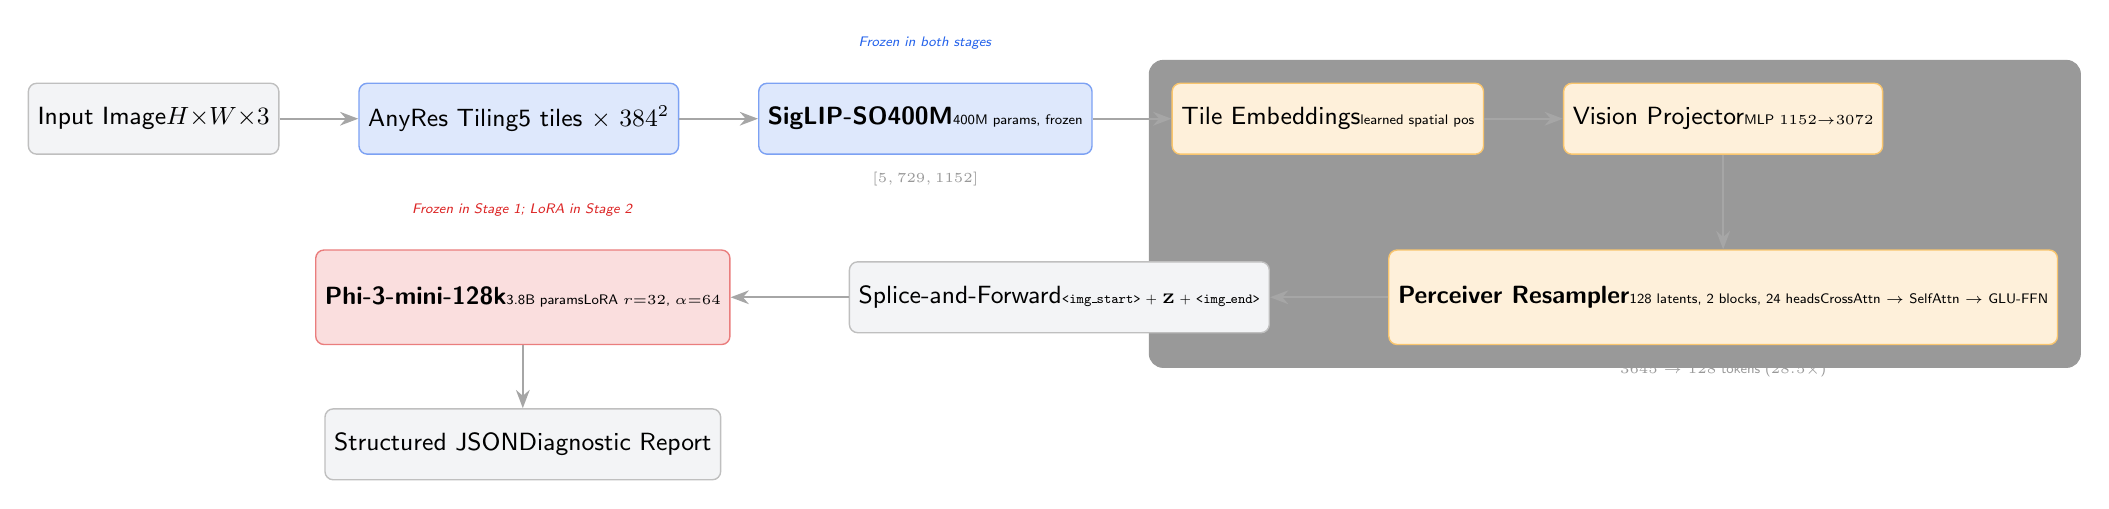
\begin{tikzpicture}[
    >=Stealth,
    node distance=0.6cm and 1.0cm,
    block/.style={
        rectangle, draw, rounded corners=3pt, minimum height=0.9cm,
        text centered, font=\small\sffamily, line width=0.5pt
    },
    vblock/.style={block, fill=visionblue!15, draw=visionblue!60},
    bblock/.style={block, fill=bridgeorange!15, draw=bridgeorange!60},
    lblock/.style={block, fill=llmred!15, draw=llmred!60},
    gblock/.style={block, fill=lightgray, draw=gray!50},
    arrow/.style={->, thick, color=gray!70},
    label/.style={font=\tiny\sffamily, color=gray!80},
]

% ── Input ──────────────────────────────────────────────────────────────────
\node[gblock, minimum width=2.2cm] (input) {Input Image\\$H{\times}W{\times}3$};

% ── AnyRes Tiling ─────────────────────────────────────────────────────────
\node[vblock, right=1.0cm of input, minimum width=2.4cm] (tiling)
    {AnyRes Tiling\\5 tiles $\times$ $384^2$};

% ── SigLIP ────────────────────────────────────────────────────────────────
\node[vblock, right=1.0cm of tiling, minimum width=2.8cm] (siglip)
    {\textbf{SigLIP-SO400M}\\{\tiny 400M params, frozen}};
\node[label, below=0.1cm of siglip] {$[5, 729, 1152]$};

% ── Tile Embeddings ───────────────────────────────────────────────────────
\node[bblock, right=1.0cm of siglip, minimum width=2.4cm] (tile_emb)
    {Tile Embeddings\\{\tiny learned spatial pos}};

% ── Vision Projector ──────────────────────────────────────────────────────
\node[bblock, right=1.0cm of tile_emb, minimum width=2.4cm] (projector)
    {Vision Projector\\{\tiny MLP $1152{\to}3072$}};
\node[label, below=0.1cm of projector] {$[3645, 3072]$};

% ── Perceiver Resampler ──────────────────────────────────────────────────
\node[bblock, below=1.2cm of projector, minimum width=3.0cm, minimum height=1.2cm]
    (perceiver) {\textbf{Perceiver Resampler}\\{\tiny 128 latents, 2 blocks, 24 heads}\\{\tiny CrossAttn $\to$ SelfAttn $\to$ GLU-FFN}};
\node[label, below=0.1cm of perceiver] {$3645 \to 128$ tokens ($28.5\times$)};

% ── Splice-and-Forward ───────────────────────────────────────────────────
\node[gblock, left=1.5cm of perceiver, minimum width=2.8cm] (splice)
    {Splice-and-Forward\\{\tiny \texttt{<img\_start>} + $\mathbf{Z}$ + \texttt{<img\_end>}}};

% ── Phi-3 ────────────────────────────────────────────────────────────────
\node[lblock, left=1.5cm of splice, minimum width=3.0cm, minimum height=1.2cm]
    (phi3) {\textbf{Phi-3-mini-128k}\\{\tiny 3.8B params}\\{\tiny LoRA $r{=}32$, $\alpha{=}64$}};

% ── Output ───────────────────────────────────────────────────────────────
\node[gblock, below=0.8cm of phi3, minimum width=2.8cm] (output)
    {Structured JSON\\Diagnostic Report};

% ── Arrows ───────────────────────────────────────────────────────────────
\draw[arrow] (input) -- (tiling);
\draw[arrow] (tiling) -- (siglip);
\draw[arrow] (siglip) -- (tile_emb);
\draw[arrow] (tile_emb) -- (projector);
\draw[arrow] (projector) -- (perceiver);
\draw[arrow] (perceiver) -- (splice);
\draw[arrow] (splice) -- (phi3);
\draw[arrow] (phi3) -- (output);

% ── Brace for Perception Bridge ─────────────────────────────────────────
\begin{scope}[on background layer]
    \node[draw=bridgeorange!40, fill=bridgeorange!5, rounded corners=5pt,
          fit=(tile_emb)(projector)(perceiver), inner sep=8pt,
          label={[font=\small\sffamily\bfseries, text=bridgeorange!80]above:Perception Bridge ($\sim$50M)}] {};
\end{scope}

% ── Stage labels ─────────────────────────────────────────────────────────
\node[font=\tiny\sffamily, color=visionblue, above=0.3cm of siglip]
    {\textit{Frozen in both stages}};
\node[font=\tiny\sffamily, color=llmred, above=0.3cm of phi3]
    {\textit{Frozen in Stage 1; LoRA in Stage 2}};

\end{tikzpicture}
\caption{\textbf{AgriPerceiver architecture.} An input leaf image is
tiled into 5 spatial regions, encoded by frozen SigLIP-SO400M, enriched
with learned tile-position embeddings, projected to the LLM dimension,
and compressed from 3,645 to 128 tokens by the Perceiver Resampler.
The compressed latents are spliced into Phi-3-mini's input sequence
for autoregressive generation of structured diagnostic JSON.}
\label{fig:architecture}
\end{figure*}


\subsection{AnyRes Spatial Tiling}

Given an input image $I \in \mathbb{R}^{H \times W \times 3}$, we
generate 5 tiles: 4 quadrant crops and 1 globally resized view, each
at $384 \times 384$ resolution. This produces patch features
$\mathbf{V} \in \mathbb{R}^{5 \times 729 \times 1152}$ from SigLIP
($729 = 27 \times 27$ patches per tile).

\subsection{Perception Bridge}

\paragraph{Tile Embeddings.}
Each tile $t \in \{1, \ldots, 5\}$ receives a learned spatial embedding
$\mathbf{e}_t \in \mathbb{R}^{1152}$, added to all patch features
within that tile to encode absolute spatial position.

\paragraph{Vision Projector.}
A two-layer MLP with GELU activation projects features from the vision
dimension ($d_v = 1152$) to the LLM dimension ($d_l = 3072$):
\begin{equation}
    \mathbf{V}' = \text{MLP}(\mathbf{V}) \in \mathbb{R}^{3645 \times 3072}
\end{equation}
where $3645 = 5 \times 729$ is the total visual token count.

\paragraph{Perceiver Resampler.}
We use $L = 128$ learned latent queries
$\mathbf{Q} \in \mathbb{R}^{128 \times 3072}$ that attend to the
projected visual features through $D = 2$ blocks of:
\begin{align}
    \mathbf{Z}^{(d)} &= \text{CrossAttn}(\mathbf{Z}^{(d-1)}, \mathbf{V}') \\
    \mathbf{Z}^{(d)} &= \text{SelfAttn}(\mathbf{Z}^{(d)}) \\
    \mathbf{Z}^{(d)} &= \text{GLU-FFN}(\mathbf{Z}^{(d)})
\end{align}
with RMSNorm and residual connections, achieving
$3645 \to 128$ compression ($28.5\times$).

\subsection{Splice-and-Forward}

The compressed latents replace the \texttt{<image>} token in the
text input:
\begin{equation}
    \mathbf{X} = [\mathbf{x}_{<\text{img\_start}}; \mathbf{Z}^{(D)}; \mathbf{x}_{>\text{img\_end}}]
\end{equation}
This hybrid sequence is then processed by Phi-3's causal attention.

\subsection{Two-Stage Training}

\paragraph{Stage 1: Alignment.}
We train only the perception bridge ($\sim$50M parameters) on
image-caption pairs with cross-entropy loss, learning rate $10^{-4}$,
for 2 epochs. Both backbones are frozen.

\paragraph{Stage 2: Specialization.}
We attach LoRA adapters ($r{=}32$, $\alpha{=}64$) to Phi-3's
\texttt{qkv\_proj}, \texttt{o\_proj}, \texttt{gate\_up\_proj},
\texttt{down\_proj}, and \texttt{up\_proj} modules. The bridge and LoRA
adapters ($\sim$85M total) are trained with sample-weighted cross-entropy
on 101K structured JSON labels for 3 epochs with gradient accumulation
($k{=}2$).

% ╔═══════════════════════════════════════════════════════════════════════════╗
% ║ 4. DATA PIPELINE                                                         ║
% ╚═══════════════════════════════════════════════════════════════════════════╝

\section{Data Pipeline}
\label{sec:data}

\subsection{Automated Labeling}

We curate 117,635 agricultural leaf images from public datasets and
generate structured diagnostic labels using Gemma-3-12B-IT (4-bit NF4
quantization). Each label contains seven fields: diagnosis,
pathology type, severity (0--1), confidence, symptoms, reasoning, and
recommended actions. After confidence-based filtering, 101,301 samples
(86\%) pass quality thresholds.

\subsection{Quality Control}

Samples are stratified by difficulty into three buckets (easy/medium/hard)
with associated sample weights used during Stage~2 training.

% ╔═══════════════════════════════════════════════════════════════════════════╗
% ║ 5. EVALUATION                                                            ║
% ╚═══════════════════════════════════════════════════════════════════════════╝

\section{Evaluation Framework}
\label{sec:eval}

% ── Fill with actual numbers after GPU runs ────────────────────────────────

\subsection{Metrics}

We evaluate across four categories (\Cref{tab:metrics}):

\begin{table}[h]
\centering
\caption{Evaluation metrics for structured agricultural diagnosis.}
\label{tab:metrics}
\small
\begin{tabular}{@{}ll@{}}
\toprule
\textbf{Category} & \textbf{Metrics} \\
\midrule
Structural & JSON validity, schema compliance \\
Classification & Type F1 (macro/weighted), diagnosis match \\
Regression & Severity MAE, RMSE, Pearson $r$ \\
Semantic & BERTScore (symptoms, reasoning, actions) \\
Expert & LLM-as-judge (5 axes, multi-consensus) \\
\bottomrule
\end{tabular}
\end{table}

\subsection{Baselines}

We compare against three general-purpose VLMs:
(1)~Gemma-3-12B-IT~\cite{team2024gemma} (the labeling model itself),
(2)~LLaVA-NeXT-7B~\cite{liu2024llavanext}, and
(3)~InternVL2-8B~\cite{chen2024internvl}.

\subsection{Results}

% ── PLACEHOLDER: Replace with actual results table ─────────────────────────

\begin{table}[h]
\centering
\caption{Main results on the held-out test set (5,062 samples).}
\label{tab:main_results}
\small
\begin{tabular}{@{}lcccccc@{}}
\toprule
\textbf{Model} & \textbf{JSON\%} & \textbf{Schema\%} & \textbf{Type F1} & \textbf{Sev. MAE} & \textbf{BERT-F1} & \textbf{Composite} \\
\midrule
LLaVA-NeXT-7B   & --  & --  & --  & --   & --  & -- \\
InternVL2-8B     & --  & --  & --  & --   & --  & -- \\
Gemma-3-12B-IT   & --  & --  & --  & --   & --  & -- \\
\midrule
\textbf{\ours{}} & --  & --  & --  & --   & --  & -- \\
\bottomrule
\end{tabular}
\end{table}

% ── PLACEHOLDER: Replace with ablation table ───────────────────────────────

\subsection{Ablation Study}

\begin{table}[h]
\centering
\caption{Ablation study on the AgriPerceiver perception bridge.}
\label{tab:ablation}
\small
\begin{tabular}{@{}lcc@{}}
\toprule
\textbf{Variant} & \textbf{Composite} & $\Delta$ \\
\midrule
Full model                     & -- & -- \\
\quad$-$ Perceiver (direct proj.) & -- & -- \\
\quad$-$ AnyRes (single tile)     & -- & -- \\
\quad$-$ Tile embeddings          & -- & -- \\
\quad$-$ Stage 2 LoRA             & -- & -- \\
Latents: 64                    & -- & -- \\
Latents: 256                   & -- & -- \\
\bottomrule
\end{tabular}
\end{table}

% ╔═══════════════════════════════════════════════════════════════════════════╗
% ║ 6. ANALYSIS                                                              ║
% ╚═══════════════════════════════════════════════════════════════════════════╝

\section{Analysis}
\label{sec:analysis}

\paragraph{Training Dynamics.}
\Cref{fig:training_curves} shows the loss curves for both training stages.
Stage~1 alignment converges rapidly from 5.0 to $\sim$0.47 over 14.7K steps,
indicating efficient bridge learning. Stage~2 specialization shows further
reduction from 0.41 to $\sim$0.04 over 37.9K steps across 3 epochs.

\begin{figure}[h]
    \centering
    
\includegraphics[width=\linewidth]{figures/training_curves.pdf}
    \caption{Training loss curves. \textbf{Left:} Stage 1 alignment
    (bridge only). \textbf{Right:} Stage 2 specialization (bridge + LoRA).
    Light traces show raw batch loss; bold lines show EMA-smoothed loss.}
    \label{fig:training_curves}
\end{figure}

% ── PLACEHOLDER: Add qualitative examples ──────────────────────────────────

% ╔═══════════════════════════════════════════════════════════════════════════╗
% ║ 7. CONCLUSION                                                            ║
% ╚═══════════════════════════════════════════════════════════════════════════╝

\section{Conclusion}
\label{sec:conclusion}

We presented \ours{}, a domain-specialized VLM for agricultural pathology
that achieves [strong/competitive] diagnostic performance while using
28.5$\times$ visual token compression and only $\sim$2\% trainable
parameters in the specialization stage. Our perception bridge, combining
AnyRes tiling, learned spatial embeddings, and Perceiver Resampling,
provides an efficient and modular approach to adapting general-purpose
foundation models for structured scientific outputs.

\paragraph{Limitations.}
Ground-truth labels are generated by Gemma-3-12B-IT rather than
domain experts, introducing potential systematic biases. Our evaluation
on severity scoring relies on silver-standard annotations. Future work
should incorporate agronomist-validated gold labels for a subset.

\paragraph{Future Work.}
We plan to extend \ours{} to multi-image longitudinal disease tracking,
integrate with precision agriculture APIs, and explore cross-crop
transfer learning.

% ╔═══════════════════════════════════════════════════════════════════════════╗
% ║ REFERENCES                                                               ║
% ╚═══════════════════════════════════════════════════════════════════════════╝

\bibliography{references}
\bibliographystyle{icml2024}

% ╔═══════════════════════════════════════════════════════════════════════════╗
% ║ APPENDIX                                                                 ║
% ╚═══════════════════════════════════════════════════════════════════════════╝

\appendix

\section{Diagnostic Report Schema}
\label{app:schema}

\begin{verbatim}
{
  "diagnosis": str,
  "type": "fungal"|"bacterial"|"viral"|
          "pest"|"deficiency"|"unknown",
  "severity": float [0.0, 1.0],
  "confidence": float [0.0, 1.0],
  "symptoms": [str, ...],
  "reasoning": str,
  "recommended_actions": [str, ...]
}
\end{verbatim}

\section{Training Hyperparameters}
\label{app:hyperparams}

\begin{table}[h]
\centering
\caption{Hyperparameters for both training stages.}
\small
\begin{tabular}{@{}lcc@{}}
\toprule
\textbf{Parameter} & \textbf{Stage 1} & \textbf{Stage 2} \\
\midrule
Learning rate   & $10^{-4}$  & $10^{-4}$ \\
Optimizer       & AdamW      & AdamW \\
Batch size      & 16         & 8 \\
Grad. accumulation & 1       & 2 \\
Epochs          & 2          & 3 \\
LoRA rank $r$   & --         & 32 \\
LoRA $\alpha$   & --         & 64 \\
LoRA dropout    & --         & 0.1 \\
Precision       & bf16       & bf16 \\
Seed            & 42         & 42 \\
\bottomrule
\end{tabular}
\end{table}

\section{Data Pipeline Details}
\label{app:data}

\begin{table}[h]
\centering
\caption{Dataset statistics.}
\small
\begin{tabular}{@{}lr@{}}
\toprule
\textbf{Statistic} & \textbf{Count} \\
\midrule
Total images           & 117,635 \\
Post-filtering (train) & 96,239 \\
Test split             & 5,062 \\
Disease types          & 6 \\
Severity range         & [0.0, 0.8] \\
\bottomrule
\end{tabular}
\end{table}

\end{document}
